% Created 2014-11-25 Tue 19:36
\documentclass[9pt,b5paper]{article}
\usepackage{graphicx}
\usepackage{xcolor}
\usepackage{xeCJK}
\usepackage{longtable}
\usepackage{float}
\usepackage{textcomp}
\usepackage{geometry}
\geometry{left=0cm,right=0cm,top=0cm,bottom=0cm}
\usepackage{multirow}
\usepackage{multicol}
\usepackage{listings}
\usepackage{algorithm}
\usepackage{algorithmic}
\usepackage{latexsym}
\usepackage{natbib}
\usepackage{fancyhdr}
\usepackage[xetex,colorlinks=true,CJKbookmarks=true,linkcolor=blue,urlcolor=blue,menucolor=blue]{hyperref}


\lstset{language=c++,numbers=left,numberstyle=\tiny,basicstyle=\ttfamily\small,tabsize=4,frame=none,escapeinside=``,extendedchars=false,keywordstyle=\color{blue!70},commentstyle=\color{red!55!green!55!blue!55!},rulesepcolor=\color{red!20!green!20!blue!20!}}
\author{Jenny Huang}
\date{\today}
\title{Android App Programming Directed Study \textasciitilde{} DrawingFun}
\hypersetup{
  pdfkeywords={},
  pdfsubject={},
  pdfcreator={Emacs 24.3.1 (Org mode 8.2.7c)}}
\begin{document}

\maketitle
\tableofcontents


\section{Checkin for 11/17/2014}
\label{sec-1}
\subsection{Buttons I have worked on}
\label{sec-1-1}
\begin{itemize}
\item openBtn for loading an image file as an ImageView
\item Undo/Redo
\end{itemize}
\subsection{Functionalities and References}
\label{sec-1-2}
\subsubsection{openBtn for loading an image file as an ImageView}
\label{sec-1-2-1}
\begin{itemize}
\item The method I applied is memory saving for AsyncTask, which is better than load images directly, which could potentially block UI for couple of seconds;
\item Loaded an image from online, but would like to try load internal images from device later on, like a drawing which I saved earlier onto my internal device;
\item Potentially apply layer oncepts to produce multiple layer drawing, needs suggestions to organize my idea how to implement this feature.
\item \textbf{Question}: Right now, my image is an ImageView in my layout, what ideas that I could use to set/change/transfer my ImageView to be my draw view background?
\item References:

\url{http://www.learn2crack.com/2014/06/android-load-image-from-internet.html}

\url{http://stackoverflow.com/questions/5776851/load-image-from-url}

\url{https://github.com/koush/UrlImageViewHelper}
\end{itemize}

\subsubsection{Undo/Redo}
\label{sec-1-2-2}
\begin{itemize}
\item After implemented subclass SuperActivity class which extends Activity on week checkin for 11/10/2014 for my ListView implementation, subclass of Path() was very difficult for me to think about implement before, but after my trial on ListView, super/sub class in Java all made sense to me now. It's a piece of cake, and I know I can wrap whatever material I need in order to paint nice and neat.
\item Implemented by developing a subclass myPath to wrap the super Path(), drawPaint color, and drawPaint strokesize together as an object.
\item Based on previous progress that I can undo/redo only with all the drawCanvas with the same paint color, now my updo/redo paths could be colorful and with various strokesizes.
\item References:

Path() library:

\url{http://grepcode.com/file/repository.grepcode.com/java/ext/com.google.android/android/2.3.1_r1/android/graphics/Path.java}

Bitmap cacheing:

\url{http://stackoverflow.com/questions/3406910/efficient-2d-drawing-in-android/3408641#3408641}

\item \textbf{Questions}: 

\begin{enumerate}
\item Undo/Redo for simple path seem to behavor fairly ok, but instead of lineTo wired line, how do I implement smooth line? How could I differentiate different strokesizes more clear with lines I have so far?

\item One little detail though, I dras after touch up, my paint color change delayed, how do I implement \textbf{real time}?

\textbf{Answered}: drawPath.reset() produced all the trouble.

\item About previous ListView six different shapes, with Undo/Redo properly functionaing, I realize I just lost my siz shapes again cause I need to rewrite/implement methods in order for them to be able to Undo/Redo \textasciitilde{}? (My subclass works perfectly for this propose, just that I lost my internal link to primitives, which means I probably should rewrite my primitives draw methods according to undo/redo prerequirements. I don't think it will be difficult, but I don't have enough time for this for the pass week, and I need to organize my ideas about these implementation clear. )

\item I prioritize undo/redo to be more important than any other buttons cause I know they would give me great practise together with primitives implementation methods rewrite. So I have not touch "Erase Rectangle" button and "paint fill" button yet. According to these idea, I would prioritize Rectangle rewrite with the highest priority, so that later on I can follow up with erase Rectangle (which means draw Rectangle first, fill with background color, and undo could remove this erase step). Correct me if I am wrong.
\end{enumerate}
\end{itemize}

\subsubsection{References: all about Android}
\label{sec-1-2-3}
\begin{itemize}
\item \url{https://github.com/kesenhoo/android-training-course-in-chinese}
\end{itemize}

\subsection{Snapshot}
\label{sec-1-3}
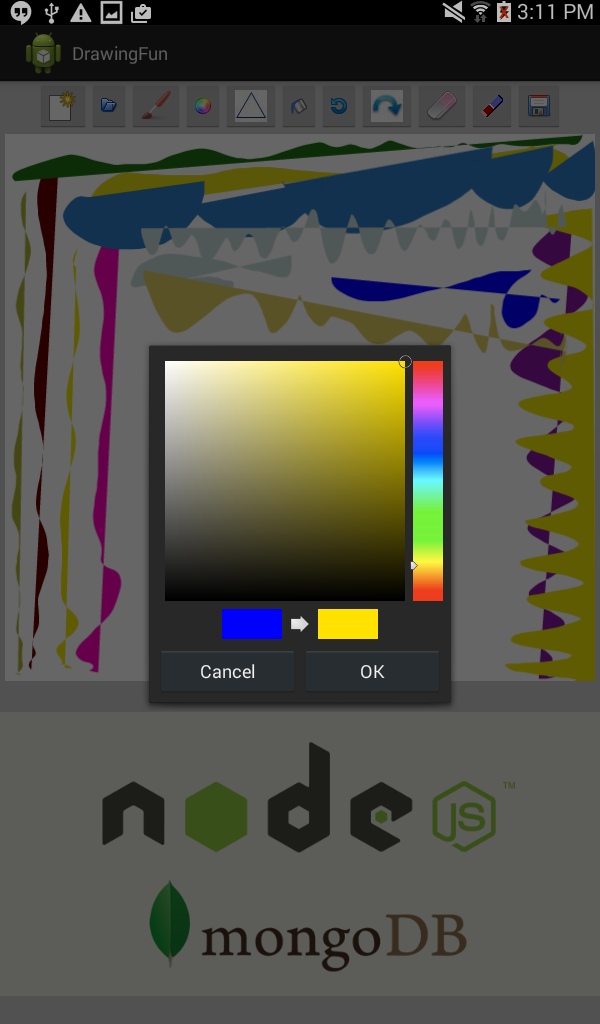
\includegraphics[width=.9\linewidth]{./Screenshot_2014-11-17-15-11-20.png}
\subsection{Todo}
\label{sec-1-4}
Only two button left untouched, could do the following or anything I am interested to implement. 
\begin{itemize}
\item Erase Rectangle
\item Fill paint
\end{itemize}

Potential interests: may implement depends on how I spend thanksgiving \textasciitilde{}~
\begin{itemize}
\item touch ImageView Activities: zoomin, zoomout, rotate, fading, etc
\item SurfaceView rotate images through new thread
\item canvas save() and restore()
\item OpenGL spinning circle
\item widely used draw methods
\item Easy draw operations
\end{itemize}

\section{Checkin for 11/10/2014}
\label{sec-2}
\subsection{Buttons I have worked on}
\label{sec-2-1}
\subsubsection{shapeBtn for primitives}
\label{sec-2-1-1}

\subsection{Functionalities and References}
\label{sec-2-2}
\subsubsection{shapeBtn for primitives: Drawing shapes with Finger for primitives}
\label{sec-2-2-1}
\begin{itemize}
\item refer to the reference below for some basic shapes: line, smooth line, circle, triangle, Rectangle, square
\item \url{http://gmariotti.blogspot.com/2014/01/drawing-shapes-with-fingers.html}
\item \textbf{ListView} in \textbf{Alert Dialog} is searched from online without direct reference.
\item Since the erase was using draw smooth line. This button works also means that I could erase a "\textbf{Rectangle}" shape, or "\textbf{Circle}" shape.
\item I have other course priority for the passed week, so I just have enough time to finish this course's priority, but I will try to work harder in order to finish all the functionalities for this course.
\item It's not a good looking ListView, but yet it's a fully functional button.
\item This button right now is fully functional, but to finish this project first, I have not spent any quality time to expand any primitives yet, rather than the existing six ones from the reference listed below.
\end{itemize}
\subsection{Snapshot}
\label{sec-2-3}
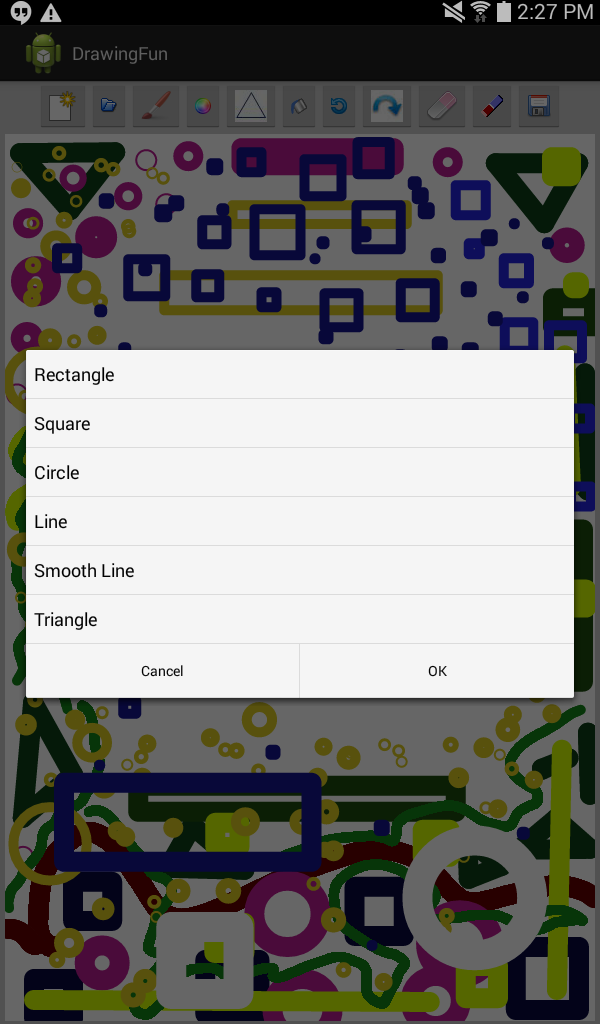
\includegraphics[width=.9\linewidth]{./20141110-14-27-05.png}
\subsection{Special Situation}
\label{sec-2-4}
\begin{itemize}
\item There were too many students piled/lined up in front of Dr. Jeffery's door, and he didn't break the line by stating that it's our direct study time. So the other classmate and I just stepped away from his office, and we didn't really meet during last week.
\item The other classmate and I have talked, and we happened to have worked on the same shapeBtn, I applied ListView in a dialog box with all six drawing shapes applied, and he created a (ListView? not sure) with a clickable button as one element with four shapes applied. And he agreeed my ListView looked way prettier than his buttons did.
\item But I am willing to and more than happy to think that he could have worked on something else important for him that I actually didn't have time to work on during the passed week.
\end{itemize}
\subsection{Todo}
\label{sec-2-5}
\begin{itemize}
\item Load image file button
\item Erase Rectangle
\item Undo/Redo
\item Fill paint
\end{itemize}

\section{Checkin for 11/3/2014}
\label{sec-3}
\subsection{Buttons I have worked on}
\label{sec-3-1}
\subsubsection{Color$_{\text{Picker}}$:}
\label{sec-3-1-1}
\subsubsection{Undo/Redo:}
\label{sec-3-1-2}

\subsection{Functionalities and References}
\label{sec-3-2}
\subsubsection{Color$_{\text{Picker}}$:}
\label{sec-3-2-1}
\begin{itemize}
\item Motivated by the Picasso Android app, seeing their multiple color choices, our starting point \textbf{12} fixed colors were too limited.
\end{itemize}
\subsubsection{Undo/Redo Buttons:}
\label{sec-3-2-2}
\begin{itemize}
\item Also motivated by the Picasso app, intended to work on \textbf{Undo} button, and ended up found \textbf{Redo} button could be very convenient as well.
\item needs to update these Undo/Redo methods later on, this is just the starting point most basic implementation for this button set.
\end{itemize}
\subsection{Snapshot}
\label{sec-3-3}
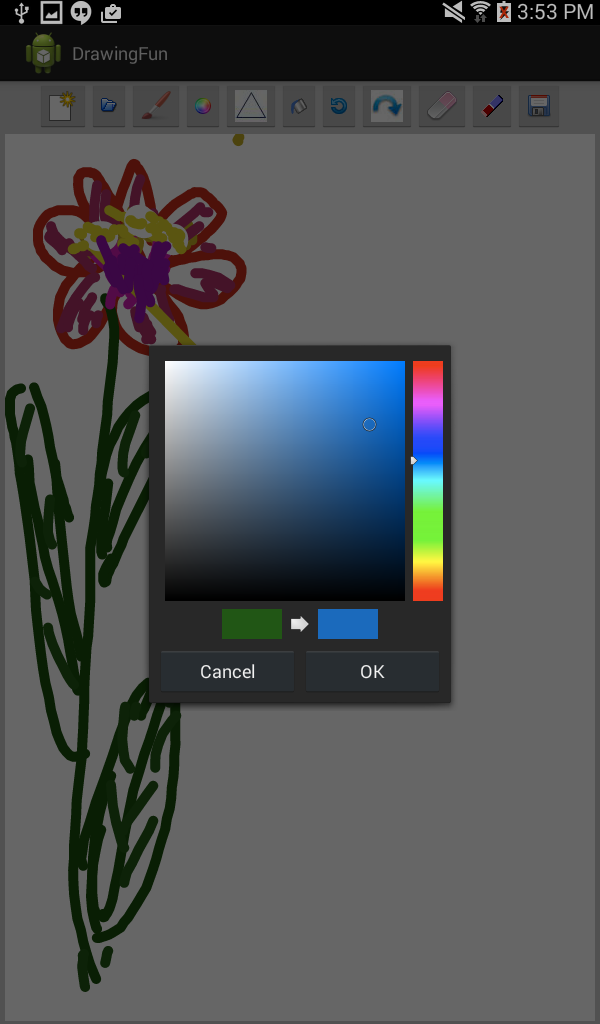
\includegraphics[width=.9\linewidth]{./20141103.png}

\subsection{Todo}
\label{sec-3-4}
\subsubsection{Drawing shapes with Finger for primitives}
\label{sec-3-4-1}
refer to the reference below: 
\begin{itemize}
\item \url{http://gmariotti.blogspot.com/2014/01/drawing-shapes-with-fingers.html}
\item This button will be first priority to finish
\end{itemize}
\subsubsection{Load image file button}
\label{sec-3-4-2}
\subsubsection{Erase Rectangle}
\label{sec-3-4-3}
\subsubsection{Undo/Redo}
\label{sec-3-4-4}
\section{first checkin 10/27/2014}
\label{sec-4}
\subsection{Goal}
\label{sec-4-1}
\begin{itemize}
\item According to the instructor's requirements that we are going to implement an simple window's Paint like Android app for later on integrating Unicon's 2D graphics to Android app.
\end{itemize}
\subsection{Course Introduction}
\label{sec-4-2}
\begin{itemize}
\item We have only two students, the other one is an udnergraduate exchange students with solid Java programming background and relatively slightly week problem-solving skills. For the first more than half semester, we used Sudoku as the starting point and tried several different topics to get our hands wet.
\end{itemize}
\subsection{Project Introduction}
\label{sec-4-3}
\begin{itemize}
\item It's after middle term already, the way we were currently trying on to make it work may just work perfectly for the other classmate, but for me, I feel like it takes forever for me to be able to make any significant progress. So about half a month ago, I was motivated and thought instead of surfacing around and having fun learning by trial and error, maybe I should start from an simple GUI app as a starting point and try my best to expend/extend the APP functionality from there. And also we would be able to work to our final project slightly earlier.
\item This GUI will be my very second GUI interface that I have ever created for my Computer Science major, (this first one was an Python Tkinter GUI one week short project for plotting graphics with data abstracted from backend database during an internship;). And I guess it may still be slightly difficult for me to start write Android App code of my own line by line, so I simply searched internet, and trying an tutorial to make a working starting point Android Paint GUI. I integrated the codes from the reference link all together, fixed minor compile errors, and it worked!
\item This "Copied" GUI will serve as the starting point, and my functionality updates start from here, and I will update my progress for this project later on by week according to the instructor's requirements and suggestions.
\end{itemize}
\subsection{References}
\label{sec-4-4}
\begin{itemize}
\item \url{http://code.tutsplus.com/tutorials/android-sdk-create-a-drawing-app-interface-creation--mobile-19021}
\end{itemize}
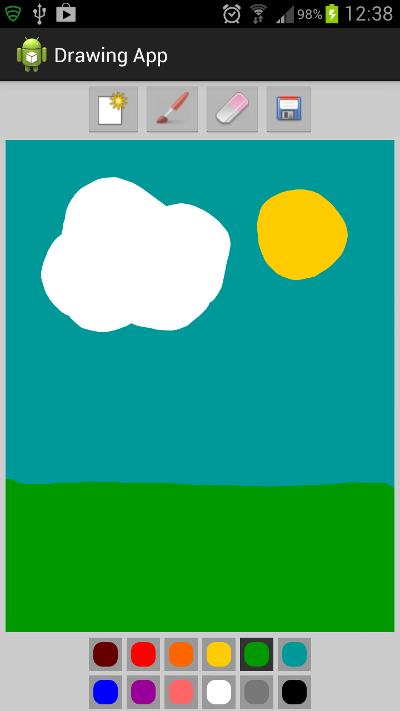
\includegraphics[width=.9\linewidth]{./android_drawing_final.png}
% Emacs 24.3.1 (Org mode 8.2.7c)
\end{document}